\documentclass[a4paper,11pt]{article}
\usepackage[utf8]{inputenc}
\usepackage{graphicx}
\usepackage{amssymb, amsmath}
\usepackage{natbib}
\begin{document}
\title{Artículo del proyecto sobre COVID-19}
\author{María Guillot Valdés}
\maketitle
\begin{center}
Resumen
\begin{center}
\begin{flushleft}
\hrefurl{https://github.com/mguillot92/proyecto_final.git}\\La pandemia de la COVID-19 ha supuesto una crisis sanitaria mundial que ha obligado a la población a introducir cambios importantes en sus comportamientos que pueden producir alteraciones en la salud mental. El objetivo es analizar síntomas depresivos y variables asociadas en población general como consecuencia del confinamiento por COVID-19.\\Palabras clave: COVID-19, confinamiento, depresión,  género, población general
\begin{flushleft}
\part{Introducción}
\begin{flushleft}
La Organización Mundial de la Salud declaró el 11 de marzo de 2020 una pandemia global debido a enfermedad por coronavirus (COVID-19) ya que afectaba a más de 100 países, con más de 100.000 casos de infectados. El 26 de marzo, el número de contagiados en el mundo alcanzaba ya el medio millón, duplicándose pocos días después (2 de abril) (OMS, 2020). El gobierno español decretó el estado de alarma el 14 de marzo para reducir la propagación de esta enfermedad y reducir la emergencia sanitaria (BOE, 2020), fecha en la que se habían computado aproximadamente 6.000 casos y 200 muertos. Desde entonces, y hasta finales de abril, las cifras ascendieron a 214.226 casos de personas infectadas y 24.415 muertes (OMS, 2020). \\
Asociado al estado de alarma se impusieron medidas drásticas y excepcionales en muchos países como en España, donde se proclamó un periodo de confinamiento obligatorio para toda la población (del 14 de marzo al 21 de junio de 2020). Dicho confinamiento implicaba permanecer refugiado el mayor tiempo posible,  así como la reducción de las interacciones sociales o la restricción de horarios de circulación. (Wilder-Smith & Freedman, 2020). Este problema ha abarcado todos los ámbitos de funcionamiento como sociedad: relacional, sanitario, económico y  educativo. 
\section{Estado del arte}
El impacto psicológico se califica de moderado a grave en la mayoría de las personas encuestadas y la probabilidad de sufrir síntomas postraumáticos y peores respuestas psicológicas incrementa cuando conviven factores individuales, sociales y demográficos: ser mujer, autopercepción de mal estado de salud, estar diagnosticado con psicopatología previa y requerir un tratamiento, trabajar en lugar de alto riesgo, preocupaciones, miedos a padecer la infección, bajo nivel educativo o la edad (Bohlken et al., 2020; Liu et al. 2020; Nguyen et al., 2020; Peng et al., 2010; Qiu et al., 2020)  
\end{flushleft}
\part{Imágenes y tablas}
	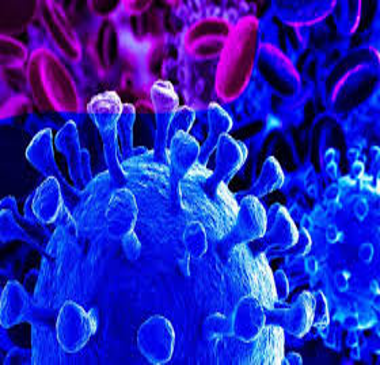
\includegraphics[width=8cm, height=5cm]{covid.png}
	
\includegraphics[width=8cm, height=5cm]{covid2.png}\\

\begin{table}[t]
\begin{center}
\begin{tabular}{| c | c | c | c | }
\hline
\multicolumn{4}{ |c| }{Coches disponibles} \\ \hline
Fabricante & Modelo & Clase & Motor \\ \hline
BMW & Serie 3 & Berlina & Diésel \\
Peugeot & 508 & Berlina & Gasolina \\
Chrysler & Voyager & Monovolumen & Gasolina \\
Land Rover & Defender & Todoterreno & Gasolina \\ \hline
\end{tabular}
\caption{Coches disponibles}
\label{tab:coches}
\end{center}
\end{table}
c
\begin{gather}
((a+b)^2 = a^2 + 2ab + b^2\\
(a-b)^2 = a^2 - 2ab + b^2\\
(a+b)(a-b) = a^2 - b^2
\end{gather}
\begin{equation}
F = ma \quad\text{Segunda ley de Newton}
\end{equation}
\begin{equation}
\label{eq:esfera}
V=\frac{4}{3}\pi r^2
\end{equation}
\part{Bibliografía}
\bibliography{biblio}
\bibliographystyle{apalike}
\nocite{Nazar2020}
\nocite{Camacho-Cardenosa2020}
\nocite{Colomo2020}
\nocite{Failoc-Rojas2020}
\nocite{Erazo20201230}
\nocite{Cassiani-Miranda2020}
\printbibliography
\end{document}
\end{document}












